\documentclass{ltjsbook}
\usepackage{docmute} 
\usepackage{myStyle} 

\begin{document}
"Practical hypothesis testing with R"
\label{chapter20}


\label{chapter20}
Until now, we have learned various statistical hypothesis testing methods, but unless we know how to apply them in practice, it will be like drawing a picture of a rice cake. This time, please deepen your understanding by actually performing null hypothesis testing using the statistical environment R. We will use R as the statistical environment and RStudio as its supplement.
There are various statistical packages available, but no matter which package or software you use, you can obtain similar output. The important thing is to understand the meaning rather than memorizing the output display location.

\section{Review of Basic Operations; Descriptive Statistics}
\subsection{Checking the Environment}
Please review how to use R and RStudio first. RStudio is an integrated environment for using R.
\paragraph{Starting RStudio} Please start RStudio. In cases such as when installing packages, administrative privileges may be required.
\paragraph{Opening a Project} RStudio can manage files and execution environments as "projects". Projects create a single folder (directory), so it is best to save script files (.R files) within it. For this class or section, please create a new project\footnote{You may reuse the project used in Chapter \ref{chapter4}.}. Once you have created or opened a project, confirm that the project is open, for example by looking at the upper right corner of RStudio ($\to$ Figure \ref{fig::20_01}).
\begin{figure}[ht]
   \centering
   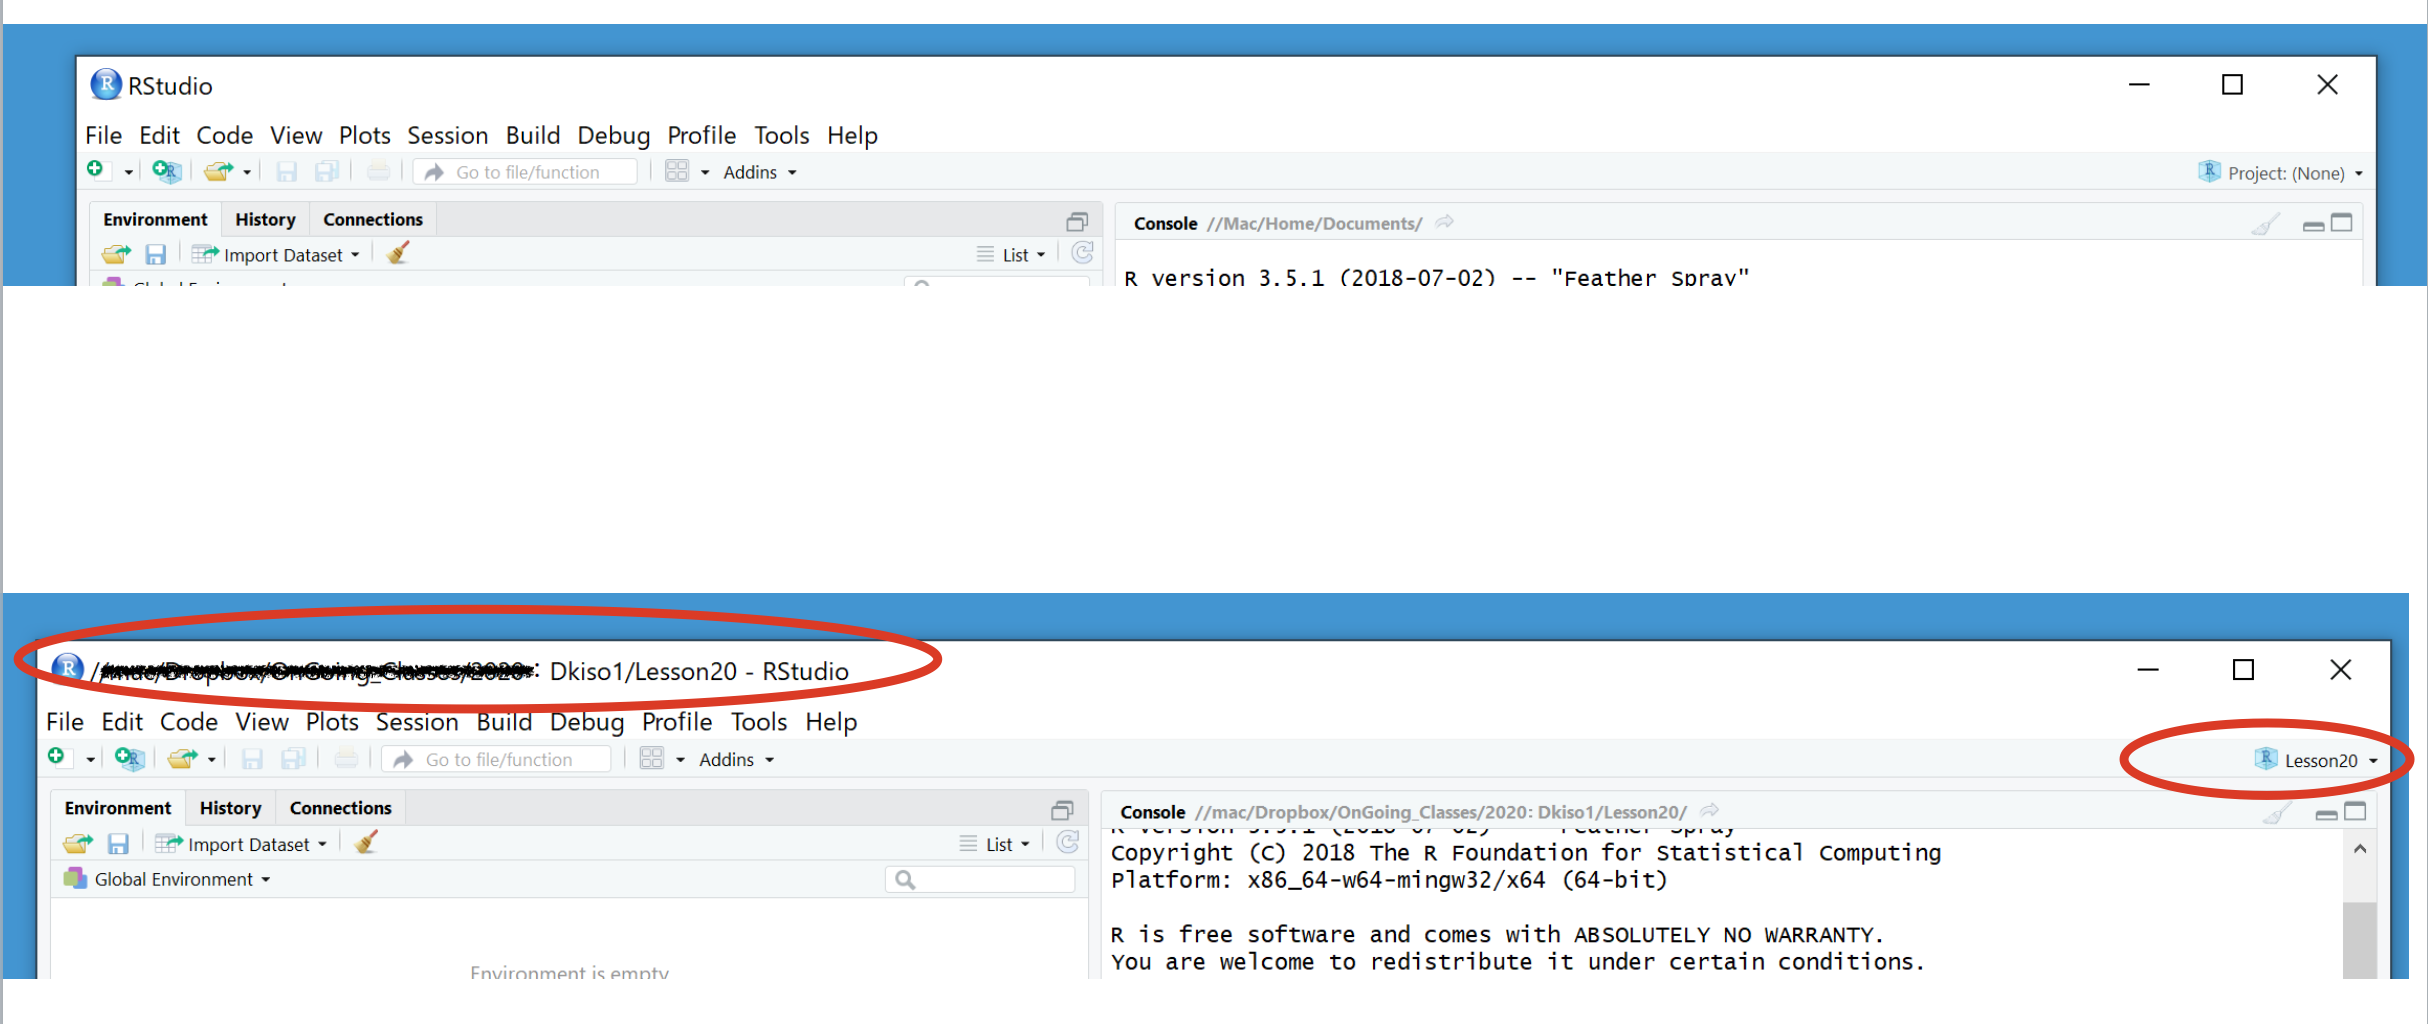
\includegraphics[keepaspectratio,width=0.8\linewidth]{../images/text20/fig20_01.png}
   \caption{プロジェクトが開いていることを確認する。上が開いていない状態。下が開いている状態。開いていると，メニューバーにフォルダが表示され，右上にプロジェクト名が表示されている。}
   \label{fig::20_01}
\end{figure}


\paragraph{Opening an R script} Prepare an R script file to write today's code. Go to \verb|File > NewFile > R Script| and display a screen with a blank R script. Once a completely blank file has opened, you are ready to go.

"Creating a dataset"
"Assigning variables to data."
As we did in Chapter \ref{chapter16}, let's practice creating a small population and taking several samples from it. Please input \texttt{code:\ref{code:20_01}}. \footnote{\# is a commented-out section that explains what calculation is being performed on that line. You do not necessarily have to enter it, however, adding comments will make it easier to read later. }

\begin{lstlisting}[language=c++,label={code:20_01},caption={繰り返しサンプリングする}]
# Clear workspace
rm(list=ls())
### 母集団を作る
X <- rnorm(100,5,1)
## 母平均
mean(X)
### 標本1を作る
s1 <- sample(X,5)
## 標本平均
mean(s1)
## 以下繰り返し
s2 <- sample(X,5)
mean(s2)
s3 <- sample(X,5)
mean(s3)
s4 <- sample(X,5)
mean(s4)
s5 <- sample(X,6)
mean(s5)
\end{lstlisting}


In R, there is a probability function where if you put \texttt{r} in front of the function name, it generates a random number. This was mentioned in Chapter 7.
The normal distribution is called \verb|normal distribution|, and in R we use the function \texttt{normal}, so normal \underline{random numbers} are written as \texttt{rnorm}. Also, since the position and width of the normal distribution change depending on the mean and standard deviation, we can make $N$ random numbers with specified mean and standard deviation by taking them as arguments\footnote{Arguments are read as "hikisuu". This refers to the numbers or options given to a function.} in \texttt{rnorm(N, mean, sd)} (I write it like this here for generalization, but actually the specific numbers are put in place of $N$, $mean$, and $sd$. For example, if you want to create 100 random numbers with a mean of 50 and a standard deviation of 10, you can write \texttt{rnorm(100, 50, 10)}.\footnote{You can also explicitly specify the arguments. Like \texttt{rnorm(n=100, mean=50, sd=10)}. In this case, there are no restrictions on the order of the arguments, so you can also write \texttt{rnorm(mean=50, n=100, sd=10)}. Conversely, if you don't specify them, they're interpreted as the number of numbers, mean, and standard deviation in order from the front.})

Now regarding this code, on the 4th line, we used the \texttt{rnorm} function to generate 100 random numbers with mean 5 and standard deviation 1. We consider this as the population. We assign it to object $X$ using the arrow symbol (\verb|<-|). As this is the population, we can calculate the population mean using the \texttt{mean(X)} function.

Next, in the \texttt{sample} function, five samples are randomly selected from the population created under the variable name \texttt{X} and assigned to an object (such as in line 8). The mean of the samples can also be calculated using the \texttt{mean} function on each object.

Please check how appropriate the sample mean is as an estimate of the population mean. Is it the case that the average of the sample means is closer to the population mean? \footnote{Since we are generating the data with random numbers, it may not always be the case. In such cases, try several times or increase the sample size of the population and sample and verify. It may be difficult to collect data from 100 people or repeat sampling many times, but it is easy to change the situation settings in a machine.}

Next, let's calculate the standard deviation (\texttt{code:\ref{code:20_01}}). Please note that the sample for s1 may differ depending on the individual execution environment, so we will not show the output here. The function for calculating the standard deviation is \texttt{sd}, and the variance can be obtained using \texttt{var}.
\begin{lstlisting}[language=c++,label={code:20_02},caption={Calculating standard deviation and variance in a function}]
# Standard deviation
sd(s1)
# Variance
var(s1)
# Square of standard deviation is equal to variance
sd(s1)^2
\end{lstlisting}

The standard deviation is the positive square root of the variance, so it has the same meaning as a statistical measure. For confirmation, the last equation is included. The symbol \texttt{\^} on line 6 represents the calculation operator for raising to a power.

By the way, I would like to draw your attention to the fact that the standard deviation (and variance) functions that R has by default are based on the unbiased variance. This means that they are calculated by dividing the sum of squared differences by n-1, not by n, where n is the total number of data points. If you want to calculate the sample variance or sample standard deviation, you need to write out the formula and calculate it yourself. Let's check it by writing the code in \texttt{code:\ref{code:20_03}}.
\begin{lstlisting}[language=c++,label={code:20_03},caption={Code for calculating sample variance}]
# Sample variance
mean((s1 - mean(s1))^2)
# Confirmation
var(s1)*4/5
\end{lstlisting}


The formula for sample variance (2nd line) consists of nested expressions. First, the mean is subtracted from the dataset $s1$ with \texttt{s1 - mean(s1)}. Although the mean is only one value, $s1$ is a vector with five elements. In such a case, R automatically reuses the mean and subtracts it from each element of $s1$. Therefore, a vector of mean deviations is created here. Then, these deviations are squared with \texttt{\^ 2}, summed, and divided by the number of elements by using the \texttt{mean} function.

In terms of confirmation, we are performing a calculation where we multiply the unbiased variance by 4 (since it is divided by $N-1=4$), and then divide by $N=5$.

\subsection{Using Probability Distribution Functions}
Next, using the example in Chapter \ref{chapter17}, let's try to calculate the probability function. Please be sure to review the difference in how to call the probability variables in R (Figure \ref{fig::20_02}).
\begin{figure}[ht]
   \centering
   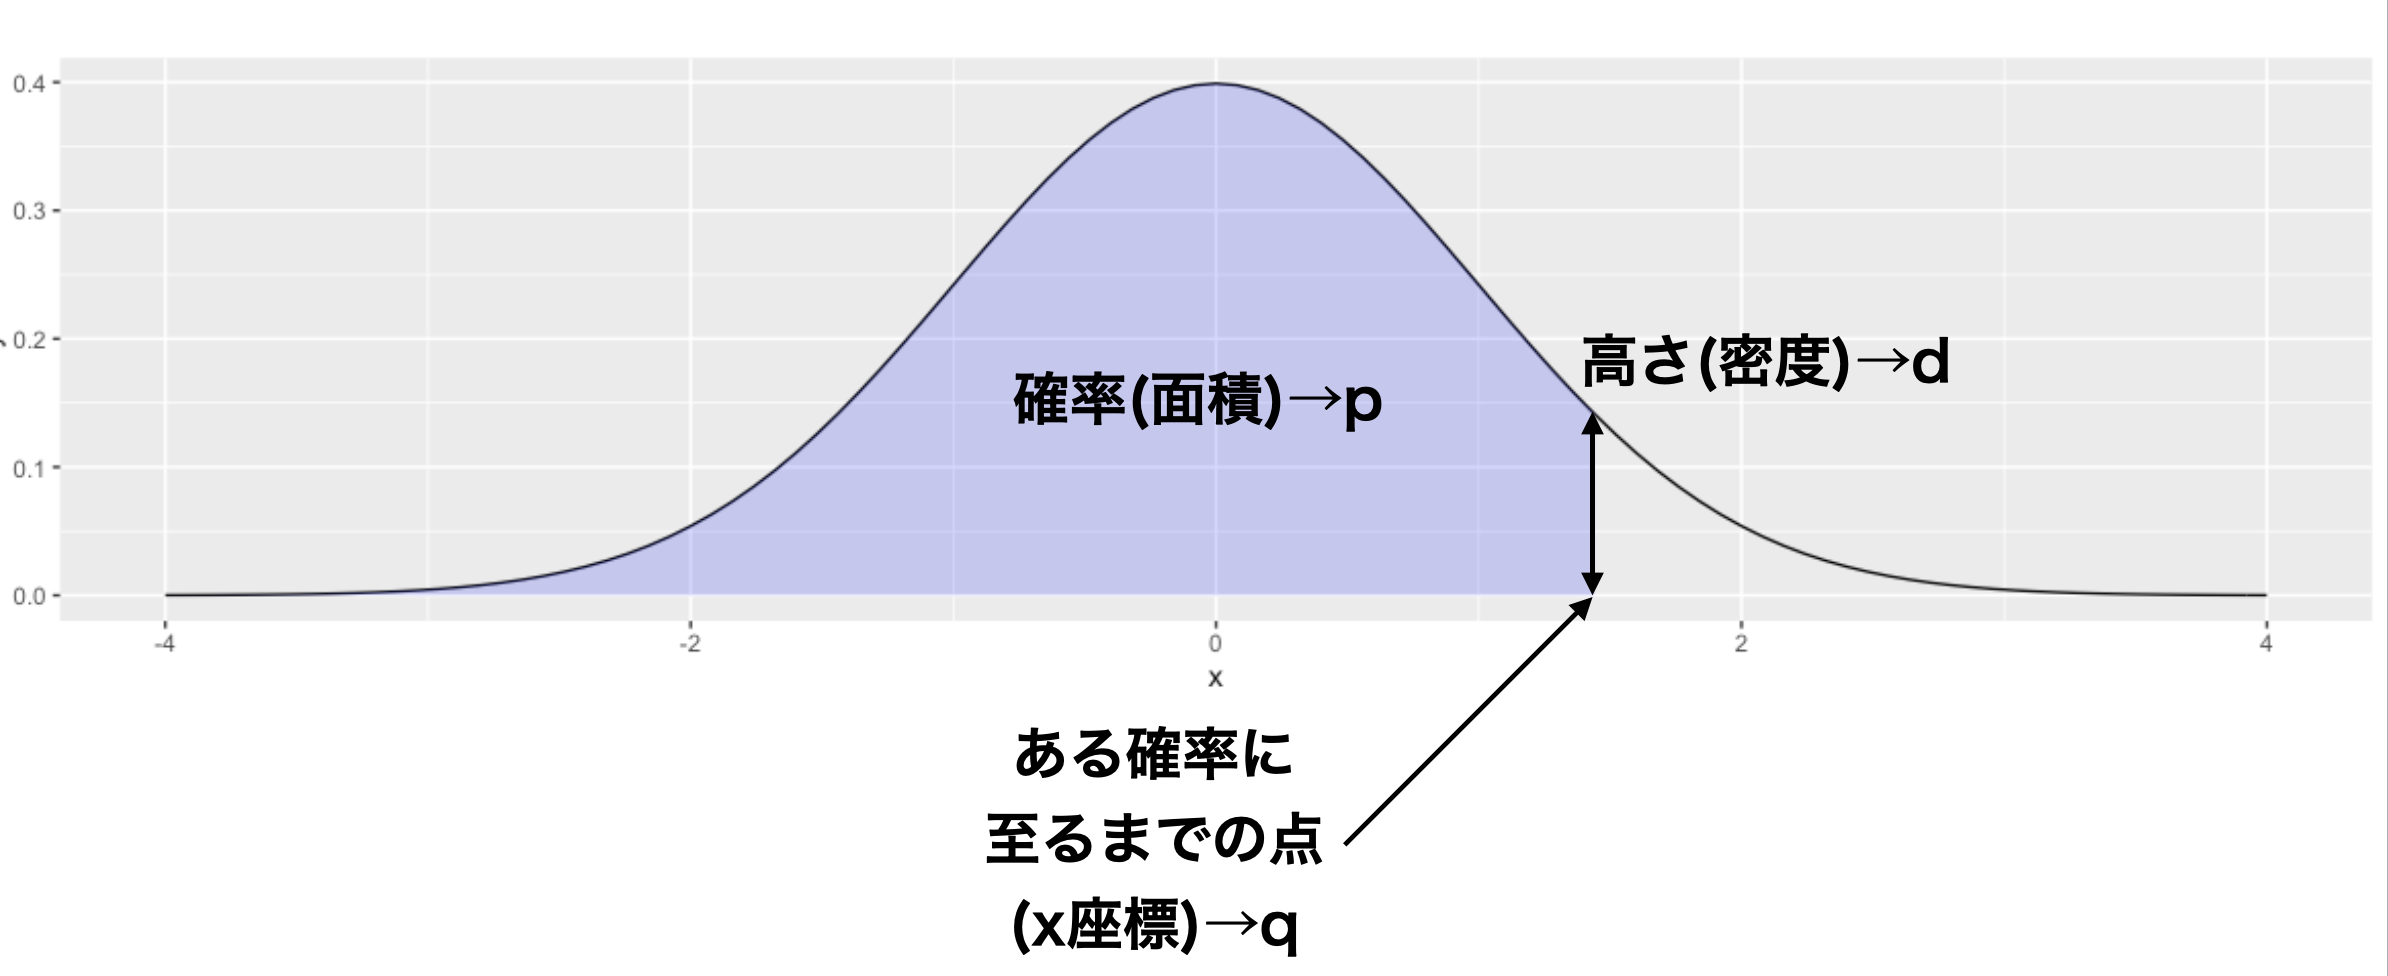
\includegraphics[keepaspectratio,width=0.8\linewidth]{../images/text20/fig20_02.png}
   \caption{Difference between \texttt{dnorm, pnorm, qnorm}}
   \label{fig::20_02}
\end{figure}


Based on this, the first step is to estimate the interval with 95% confidence interval. As we want 95% of the area around the peak, we need to have an estimate for it.
\begin{enumerate}
   \item I want a 95\% width around the peak.
   \item The total area under the probability distribution is 1, so we want to leave 5\% on both ends.
   \item That means we only need 2.5\% on one side.
   \item Since we want the x-coordinate, we will use \texttt{qnorm} to find the probability point at 97.5\% from the bottom.
\end{enumerate}

It goes through the following procedure (Figure \ref{fig::20_03}). In the code, you can use \texttt{code:\ref{code:20_04}} to be OK.
\begin{figure}[ht]
   \centering
   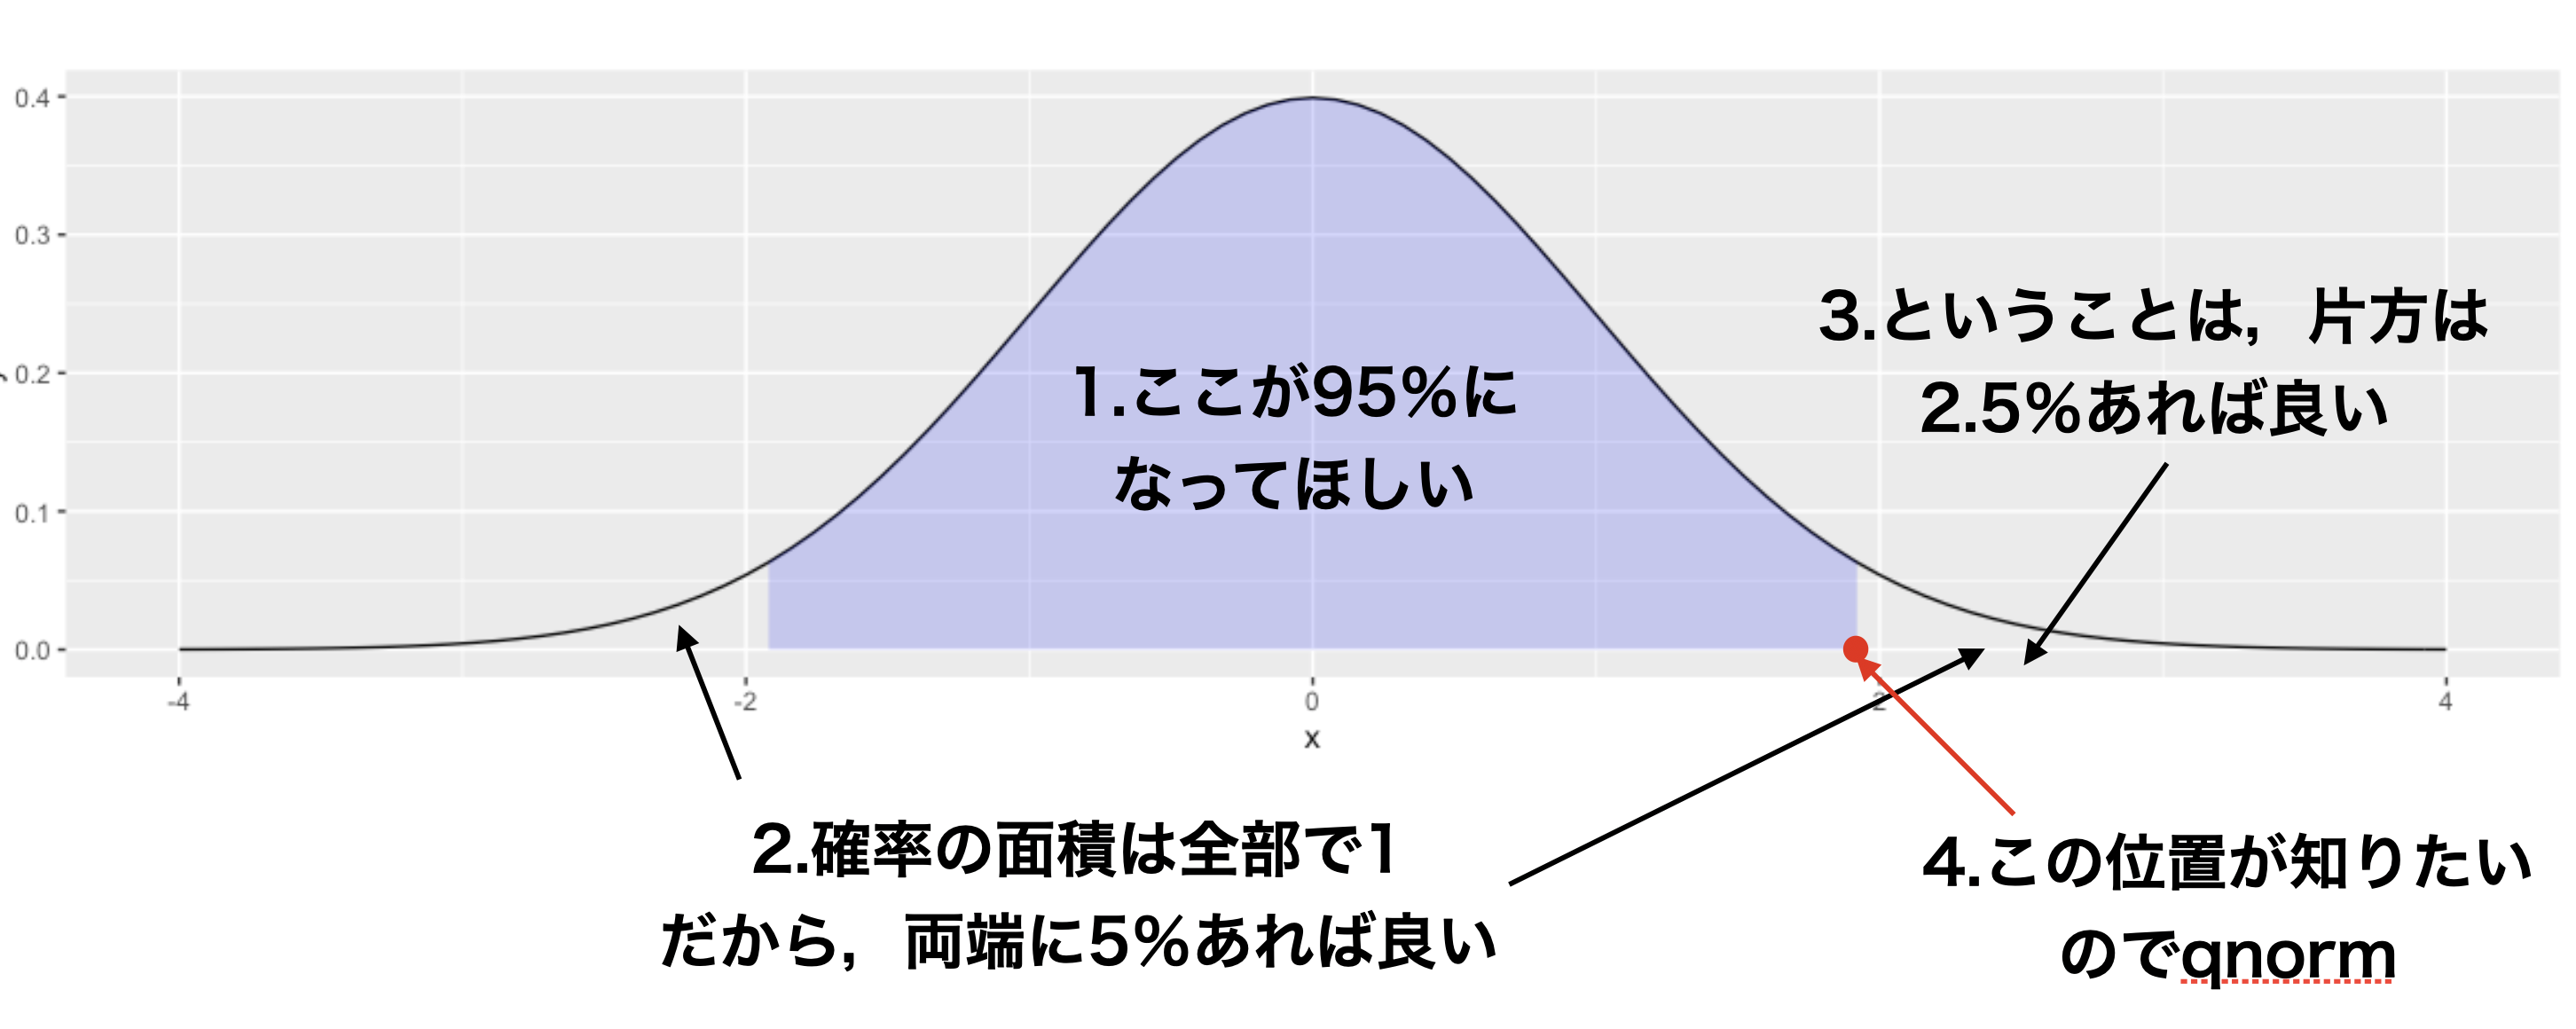
\includegraphics[keepaspectratio,width=0.8\linewidth]{../images/text20/fig20_03.png}
   \caption{Logic for finding the 95\% probability point}
   \label{fig::20_03}
\end{figure}


\begin{lstlisting}[language=c++,label={code:20_04},caption={95\% interval of the normal distribution}]
# 95% interval of the normal distribution
qnorm(0.975, mean = 0, sd = 1)
\end{lstlisting}

Let's do interval estimation with this. This time, we took a sample from a population with a mean of 5 and a standard deviation of 1. For example, if we want to do interval estimation for the first object, $s1$, we can calculate it using \texttt{code:\ref{code:20_05}}. We can represent it without a negative sign by calculating it with the probability point of 0.025 from the bottom instead of using -1.96.
\begin{lstlisting}[language=c++,label={code:20_05},caption={標本1の区間推定}]
    mean(s1)+qnorm(0.025)*(1/sqrt(5))
    mean(s1)+qnorm(0.975)*(1/sqrt(5))
\end{lstlisting}



However, this is when the population variance is known, which is not usually the case, so we use the t-distribution. In R, the function name for the t-distribution is simply "t", so by using "dt, pt, qt" etc., you can obtain the probability density, cumulative probability, and probability point. However, don't forget that the degree of freedom "df" is required as an argument. The interval estimation using this method is as shown in the following code (\texttt{code:\ref{code:20_06}}), taking note of the degree of freedom and using the sample variance \texttt{sd(s1)} in place of the population variance.
\begin{lstlisting}[language=c++,label={code:20_06},caption={母分散がわからない場合}]
    mean(s1)+qt(0.025,df=4)*(sd(s1)/sqrt(5))
    mean(s1)+qt(0.975,df=4)*(sd(s1)/sqrt(5))
\end{lstlisting}

"However, some people may find writing equations more troublesome than they thought. Actually, there is an easier way to do it. It is to use the function of t-test in R. Speaking of t-tests, you might think of testing the difference in means between two groups, but we will do that in the next section. For now, please execute \texttt{code:\ref{code:20_07}}."
\begin{lstlisting}[language=c++,label={code:20_07},caption={Estimation with the t.test function}]
    t.test(s1,mu=5,conf.level = 0.95)
\end{lstlisting}

This is a testing method for examining whether the sample mean obtained from a population with a mean of 5 significantly deviates from the population mean. When executed, in my environment, results similar to \texttt{console\ref{RS:out20_01}} were obtained\footnote{It should be noted that since sample s1 may vary depending on the execution environment, the results may differ from the numbers on your screen. It is important to understand the meaning of the output.}.

\begin{Rscreen}{Output of t-test}{out20_01}
   \begin{verbatim}
> t.test(s1,mu=5,conf.level = 0.95)

One Sample t-test

data:  s1
t = 0.92459, df = 4, p-value = 0.4075
alternative hypothesis: true mean is not equal to 5
95 percent confidence interval:
 4.154629 6.689527
sample estimates:
mean of x 
 5.422078
\end{verbatim}
\end{Rscreen}

The Japanese words used in the original TeX code are already in English.

Various outputs are being generated, but on the 5th line from the bottom, it should say 95 percent confidence interval, with \texttt{CI[4.154629,6.689527]} being shown, which is the same as the previous calculation result. Below that, please confirm that the sample mean \texttt{5.422078} is also the same result as \texttt{mean(s1)}.

By the way, this function \texttt{t.test} has default settings of \texttt{mean = 0} and \texttt{conf.level = 0.95}.

"t-Test with Correspondence"
Now, let's use the function we previously saw, \texttt{t.test}. This function, as expected, is a tool to perform t-tests. Let's try using it in a actual testing scenario.

This is about calculating a t-test with correspondence, specifically the test of the difference in means between two levels within a single factor group. In the previous section, there were complicated formulas, but this time the calculations will be done by a machine, so as usual, be sure to carefully check the output.

For example, we will use the data of 10 participants in Table \ref{fig::19_01}. Execute the code \texttt{\ref{code:20_08}} to store the original data in an object.
\begin{lstlisting}[language=c++,label={code:20_08},caption={t検定を行う}]
X <- c(34, 25, 13, 21, 13, 26, 19, 12, 19, 19)
Y <- c(35, 30, 16, 27, 20, 28, 16, 14, 18, 21)
t.test(X, Y, paired = T, alternative = "less")
\end{lstlisting}


\paragraph{Explanation of the Code}
\begin{description}
	\item[1行目] 一方のデータをオブジェクト\texttt{X}に代入しています。\texttt{c}は結合combineという関数です。
	\item[2行目] 他方のデータをオブジェクト\texttt{Y}に代入しています。
	\item[3行目] t検定を行っています。引数として，データ\texttt{X,Y}を指定し，次に\texttt{paired}オプションを\texttt{T}に\footnote{大文字の\texttt{T}は$TRUE$，真であり，この逆は\texttt{F}とかいて$FALSE$,偽を意味する\textbf{特別な文字}です。真か偽か，本当か嘘かという2つの状態を表す論理値と呼ばれるもので，ここではスイッチオン/オフの意味です。対応スイッチ，オン！という意味ですね。大文字の$T,F$をオブジェクト名にして利用することも可能ですが，Rが専門的な意味で使う予約語なので，一般的にはそのような使用は避けた方が望ましいです。}，対立仮説alternativeを「XがYよりも小さい」という\underline{片側検定}にしてあります。
\end{description}

Now, while this script was written to be easy to understand intuitively, it is also possible to express the same thing in a different way (\texttt{code:\ref{code:20_09}}).

\begin{lstlisting}[language=c++,label={code:20_09},caption={t検定その2}]
X <- c(34, 25, 13, 21, 13, 26, 19, 12, 19, 19)
Y <- c(35, 30, 16, 27, 20, 28, 16, 14, 18, 21)
dat <- data.frame(condition = c(rep(1, 10), rep(2, 10)), value = c(X, Y))
dat$condition <- factor(dat$condition, labels = c("pre", "post"))
t.test(value ~ condition, data = dat, paired = T, alternative = "less")
\end{lstlisting}

This is the same as before for the first and second lines.
\begin{description}
   \item[Line 3] Creating a data frame from objects. The values of the data are created with the variable \texttt{value} along with a conditional variable \texttt{condition} to distinguish them by conditions. The \texttt{rep} function in \texttt{condition} repeats a certain character or number, and in this case, it creates 10 ones with \texttt{rep(1,10)}. You can see this behavior clearly by running this section only (\texttt{console\ref{RS:out20_02}}).
      \begin{Rscreen}{rep output}{out20_02}
         \begin{verbatim}
> rep(1,10)
[1] 1 1 1 1 1 1 1 1 1 1
    \end{verbatim}
      \end{Rscreen}
   \item[Line 4] Replacing the previously created \texttt{condition} variable with a factor type (labeled nominal scale level).
   \item[Line 5] This is a t-test, but the format is different. We use a tilde \texttt{\~} and change the writing style to dependent variable\verb|~|independent variable.

This is a way to create a data frame, so it would be good to see what form the data frame is in (\texttt{console\ref{RS:out20_03}}).

\begin{Rscreen}{datの中身を確認}{out20_03}
   \begin{verbatim}
> dat
   condition value
1        pre    34
2        pre    25
3        pre    13
(中略)
11      post    35
12      post    30
13      post    16
(後略)
\end{verbatim}
\end{Rscreen}

During actual data analysis, it is common to read data files from an external source or analyze data that has already been formatted into a data frame. In R, it is common to represent the functional relationship between independent and dependent variables using the tilde symbol, so we have explained how to use it in both ways.

Well, the results obtained are as shown in \texttt{console\ref{RS:out20_04}}.
\begin{Rscreen}{t.testの出力}{out20_04}
   \begin{verbatim}
Paired t-test
data:  value by condition
t = -2.4783, df = 9, p-value = 0.01754
alternative hypothesis: true difference in means is less than 0
95 percent confidence interval:
        -Inf -0.6248331
sample estimates:
mean of the differences 
                   -2.4 
\end{verbatim}
\end{Rscreen}


I see that the t-value is shown on the third line from the top. The actual value of the t-statistic under the null hypothesis is $t(9)=-2.4783$, and the probability of this occurring is $p=0.01754$. The alternative hypothesis is that the true difference in means is less than 0. In the R code, this is expressed as the first variable being less than the second variable. The one-tailed test is performed because the \texttt{t.test} function was called with the argument \texttt{alternative="less"}. If \texttt{alternative="greater"} is used instead, the test would be for the opposite one-tailed test (the score for the prior data is greater than that of the posterior data). If nothing is specified (\texttt{alternative="two.sided"}), a two-tailed test is performed.

Please refer to the previous chapter ($\to$ Lecture \ref{chapter19}) to understand how to interpret these results and how to include them in your report.

"Unpaired t-test without correspondence"
Let's consider testing the difference in means between two independent groups with no corresponding response, in other words, testing data from a one-factor between-subjects (2-level design) study. Continuing from the previous chapter, let's analyze the data in Table \ref{tbl::19_02}. Without delving into complex calculations, please input \texttt{code:\ref{code:20_10}} and execute the analysis.
\begin{lstlisting}[language=c++,label={code:20_10},caption={formulaで指定}]
X <- c(25, 15, 24, 17, 22)
Y <- c(31, 28, 30, 19, 18)
dat <- data.frame(condition = c(rep(1, 5), rep(2, 5)), value = c(X, Y))
dat$condition <- factor(dat$condition, labels =  c("control","experimental"))
t.test(value ~ condition, data = dat)
\end{lstlisting}

The contents of the script are almost the same as before. The major difference is that there are no arguments for the \texttt{t.test} function, and neither the \texttt{paired} nor the \texttt{alternative} option is present. This is because the function is using the default settings. In R, the \texttt{t.test} function performs a two-sided test without pairing by default.

The result should be displayed as follows (\texttt{console\ref{RS:out20_05}}).
\begin{Rscreen}{Welch correction}{out20_05}
   \begin{verbatim}
Welch Two Sample t-test

data:  value by condition
t = -1.3506, df = 7.195, p-value = 0.2178
alternative hypothesis: true difference in means is not equal to 0
95 percent confidence interval:
 -12.609577   3.409577
sample estimates:
     mean in group control mean in group experimental 
                      20.6                       25.2 
\end{verbatim}
\end{Rscreen}

Please confirm whether the result matches the one obtained from manual calculation from the previous time.

Hmm? The degree of freedom is 7.195? Wasn't it supposed to be 8 degrees of freedom (the degree of freedom for the experimental group is $5-1=4$, the degree of freedom for the control group is also $5-1=4$, and adding the two together gives $4+4=8$)?

"Welch's correction"
That's correct, the degrees of freedom for the t-test should be 8, but it's coming out as a strange number. This is because there is another procedure involved in the test that hasn't been explained yet.

Please remember the assumptions that were made for the test. While assuming the null hypothesis that the difference in population means is zero is a hypothesis, it is also an assumption that precedes it. Specifically, the assumption was that the two groups were obtained from normal distributions, and although there is a difference in the mean values, the assumption was made that the population standard deviation was the same.

What if this assumption is violated? If we cannot assume normal distribution in the population, we cannot perform a t-test. For example, if the data pertains to differences in annual income or involves numerical figures relating to ratios or angles, we cannot assume normal distribution and therefore cannot conduct a t-test. Even if we assume normal distribution, we may need to reconsider our estimation method if the population standard deviation differs.

This problem is solved by adjusting the degrees of freedom of the t-value. The so-called t-test until now has been a calculation method for cases where the assumption of equal variance is satisfied (which also involves homogeneity of variance), and when this assumption is not met, an adjustment called \keytermE{Welch's correction}(ウェルチの補正) is necessary.

The \texttt{t.test} function in R returns, by default, the result of applying Welch's correction, which is based on a more lenient assumption. This is done to avoid having to check whether the variances are equal, which can be a cumbersome procedure. The first line of the output also states that the test used is the Welch Two Sample t-test. Using this method, the results are:
\begin{quote}
   No statistically significant difference was found between the two groups with $t(7.195)=1.351, p = 0.2178$.
\end{quote}

I report that the value of $t$, which in the case of a two-sided test does not have any meaning for the sign, has been calculated. Let's not only consider whether there is a difference, but also pay attention to the 95% confidence interval of the difference. According to the results, the 95% confidence interval for the difference was CI[-12.609577, 3.409577]. Since the range of the difference is from -12 to +3 and includes the null hypothesis that the difference = 0, it is not significant.


By the way, when assuming equal variances, you can use the options of the \texttt{t.test} function (\texttt{code:\ref{code:20_11}}).

\begin{lstlisting}[language=c++,label={code:20_11},caption={Options for Variance}]
t.test(value ~ condition, data = dat,var.equal = T)
\end{lstlisting}


With this, you can obtain results like \texttt{console\ref{RS:out20_06}}.

\begin{Rscreen}{分散が等しいという仮定を置く}{out20_06}
   \begin{verbatim}
	Two Sample t-test

data:  value by condition
t = -1.3506, df = 8, p-value = 0.2138
alternative hypothesis: true difference in means is not equal to 0
95 percent confidence interval:
 -12.453967   3.253967
sample estimates:
     mean in group control mean in group experimental 
                      20.6                       25.2 
\end{verbatim}
\end{Rscreen}

With this method, the degrees of freedom are also integers (although the determination result remains unchanged).

Verification of Post-hoc Effect Size
Although the exam is over, we are wondering if this experimental data had a "winning strategy". In other words, we are curious if the difference of the population mean in the overall population is large enough to make a significant impact. We do not know the population value, but we have been estimating it using statistical data. Therefore, let's consider after collecting the data, how large the effect size was.

It is also possible to easily calculate effect size using R. R offers various statistical functions with the addition of packages, and introducing the \textsf{effsize} package \citep{effsize} for effect sizes makes calculation simple. Please refer to chapter \ref{chapter19} for information on effect size. Here, we introduce the recommended method of calculating Hedges' g (\texttt{code:\ref{code:20_12}}).

\begin{lstlisting}[language=c++,label={code:20_12},caption={効果量を求める}]
# パッケージの読み込み
library(effsize)
cohen.d(value ~ condition, data = dat, hedges.correction = T)
\end{lstlisting}

First, in the second line, load the package\footnote{If you do not have this package, you need to download it from the internet and save it locally (on your PC). This download is called "installing a package" and can be done using the \texttt{install.packages} function. To install the package for this example, enter \texttt{install.packages("effsize")} and run it. Pay attention to capitalization! Also, you do not need to do this every time, once you download it is enough.}, and in the following line, compute the Cohen's d with Hedges' correction.

The result is shown as \texttt{console\ref{RS:out20_07}}.
\begin{Rscreen}{Output of effect size}{out20_07}
   \begin{verbatim}
Hedges's g

g estimate: -0.7715342 (medium)
95 percent confidence interval:
       lower      upper 
-2.1369693  0.5939009 
\end{verbatim}
\end{Rscreen}


As indicated by "g estimate: -0.7715342 (medium)" in the text, the estimated value is 0.77 and this is of medium size. Although there seems to be a moderate difference, it may not have been significant in this case due to the small sample size. If it had been properly designed in advance and conducted as an experimental procedure, it would have been improved.

Calculating effect size can also be done retrospectively by considering how much difference there is likely to be in the standardized mean values ​​from this sample. Of course, it can also be used to design sample sizes (considering how many samples are needed) by assuming the difference in the mean values ​​beforehand. Make sure to include the calculated sample effect size in the report.

\begin{quote}
   There was no statistically significant difference between the two groups at $t(7.195)=1.351, p=0.2178$. The effect size calculated by Hedges' g was 0.77.
\end{quote}


\subsection{Appendix}
As an appendix, I will add two points. Please read them if you have time or interest.
\paragraph{Calculating Effect Size for Paired t-test} When performing a paired $t$-test and seeking to obtain its effect size, you should turn on the paired option as shown in the following code example (\texttt{code:\ref{code:20_13}}).

\begin{lstlisting}[language=c++,label={code:20_13},caption={cohenのd}]
cohen.d(X,Y,paired = TRUE)
\end{lstlisting}

However, if you are using a writing style that includes tilde (~), when using \texttt{code:\ref{code:20_14}}, the output will display a warning message like the one shown in \texttt{console:\ref{RS:out20_08}}.
\begin{lstlisting}[language=c++,label={code:20_14},caption={cohenのdその2}]
cohen.d(value ~ condition, data = dat, paired = TRUE)
\end{lstlisting}


\begin{Rscreen}{rnorm output}{out20_08}
   \begin{verbatim}
Cohen's d

d estimate: -0.344241 (small)
95 percent confidence interval:
      lower       upper 
-0.64457930 -0.04390272 

    Warning message: 
cohen.d.formula(value ~ condition, data = dat, paired = TRUE) で: 
Trying to compute paired samples Cohen's d using formula input. Results may be incorrect
 if cases do not appear in the same order for both levels of the grouping factor. Use the
format 'value ~ treatment | Subject(id)' to specify a subject id variable.
\end{verbatim}
\end{Rscreen} 

Japanese words in the original text: 

- 警告メッセージ
- で

This warning is saying that "the variable for identifying individual correspondence is not included in the dataset, so the results may be incorrect. Please use the following format." To address this, you should use \texttt{code:\ref{code:20_15}}.
\input{text1_chap20old_escape_30}
The key point here is to create a variable to identify the ID in the 5th line. \footnote{The function \texttt{rep} repeats \texttt{1:10} twice. In R, numbers connected with a colon indicate a sequence.} We have also rewritten the formula for calculating the effect size in the proposed format of the warning.

"How to Design a Sample Size"
In an unsupported t-test, even though the effect size was 0.7, it did not show statistical significance. It was suggested that this may be due to the small sample size, but then how many pieces of data were needed? We can obtain a hint by inputting the code shown in \texttt{code:\ref{code:20_16}} into R.
\begin{lstlisting}[language=c++,label={code:20_16},caption={power.t.test function}]
power.t.test(power = 0.8, delta = 0.7, sig.level = 0.05)
\end{lstlisting}

In this code, there are no Japanese words to translate. It appears to be a code snippet in C++ that uses the power.t.test function with certain input parameters.

Here, we set \texttt{delta=0.7} based on the assumption that there is a standardized mean difference of 0.7. We used this value because it was suggested by the results of the post-hoc power analysis conducted earlier. However, it is acceptable to estimate a smaller or larger value as well. Additionally, we set \texttt{power=0.8}, which is the \textit{power} discussed in Section \ref{sec::18_05}. We aimed to reduce the Type II error (false negative) to approximately 20\% and achieve an 80\% probability of detecting a significant difference ($1-\beta=0.8$). The significance level is 5\% ($\alpha=0.05$), which is set as \texttt{sig.level=0.05} in the script.

Now, looking at the output of this, it was shown as follows (\texttt{console\ref{RS:out20_09}}).
\begin{Rscreen}{rnormの出力}{out20_09}
   \begin{verbatim}
Two-sample t test power calculation 

n = 33.02467
delta = 0.7
   sd = 1
sig.level = 0.05
power = 0.8
alternative = two.sided

NOTE: n is number in *each* group
\end{verbatim}
\end{Rscreen}

As mentioned here, if you are conducting a study with an effect size of 0.7 and a power of 0.8, you would want to gather around 33 to 34 people. However, in this case, only 5 people were gathered. This is shown in \texttt{code:\ref{code:20_17}} and \texttt{console:\ref{RS:out20_10}}.

\begin{lstlisting}[language=c++,label={code:20_17},caption={power.t.testで$n$を固定}]
power.t.test(n = 5, delta = 0.7, sig.level = 0.05)
\end{lstlisting}


\begin{Rscreen}{Output of power analysis}{out20_10}
   \begin{verbatim}
Two-sample t test power calculation 

n = 5 (sample size)
delta = 0.7 (effect size)
sd = 1 (standard deviation)
sig.level = 0.05 (significance level)
power = 0.16318 (statistical power)
alternative = two.sided (two-tailed test)

NOTE: n is number in *each* group
\end{verbatim}
\end{Rscreen}

As stated here, the statistical power is 0.16, which means that even if this study was conducted 100 times, it would correctly identify statistically significant differences only about 16 times, given a sample size of n=5. It's like playing a losing game.
\section{Task/Assignment}
Task 1: Sample Statistics and One-Sample Test.
Assuming that data like that in Table \ref{exe:20_1} has been obtained, please follow the following instructions and answer the questions about the results.
% latex table generated in R 4.0.2 by xtable 1.8-4 package
% Fri Oct 16 12:52:58 2020
\begin{table}[ht]
	\centering
	\caption{課題1}
	\label{exe:20_1}
	\begin{tabular}{rrrrrrrrrr}
		\hline
		56 & 57 & 49 & 45 & 56 & 32 & 56 & 47 & 47 & 41 \\
		\hline
	\end{tabular}
\end{table}

\begin{enumerate}
   \item Please calculate the sample variance of this dataset.
   \item Please calculate the square root of the unbiased variance of this dataset.
   \item Assuming this dataset is derived from a population that follows a normal distribution, please perform a 95\% interval estimation for the population mean.
   \item Please perform a hypothesis test at a 5\% significance level to determine if this dataset is derived from a normal distribution with a population mean of $\mu=50$.
\end{enumerate}


"Task 2: Paired t-test with corresponding data."
Please answer the following instructions regarding the results obtained from pre- and post-intervention psychological tests, as shown in Table \ref{exe:20_2}.
% latex table generated in R 4.0.2 by xtable 1.8-4 package
% Fri Oct 16 12:59:41 2020
\begin{table}[ht]
   \centering
   \caption{課題2}
   \label{exe:20_2}
   \begin{tabular}{rrrrrrrrr}
      \hline
      pre  & 19 & 38 & 24 & 25 & 12 & 28 & 11 & 17 \\
      post & 31 & 23 & 28 & 35 & 14 & 4  & 4  & 38 \\
      \hline
   \end{tabular}
\end{table}


\begin{enumerate}
   \item Determine whether the pre-score is lower than the post-score at a 5% level of significance.
\end{enumerate}


Task 3: Unpaired t-test without matching.
Please provide the table results of the psychological tests for the control group and the experimental group, as shown in Table \ref{exe:20_3}. Follow the instructions below and answer the questions regarding the results.
% latex table generated in R 4.0.2 by xtable 1.8-4 package
% Fri Oct 16 13:05:51 2020
\input{text1_chap20old_escape_39}

\begin{enumerate}
	\item 母分散が等しいと仮定したt検定を実行してください。
	\item 母分散が等しいという仮定をおかないt検定を実行してください。
	\item Hedgesのgを算出してください。
\end{enumerate}


\end{document}
